\section{\translate{Theory}}\label{sec:theory} 
In the report's theory study, sometimes called Related work, there may be
additional facts required for the reader's understanding of the report. At this
point a summary of background material in the area should be provided, i.e.\
standards, scientific articles, books, magazines, documents on the web,
technical reports and user manuals. Explain pedagogically with clear examples
and many illustrations.  It should be demonstrated that you have an awareness of
the context and the background of your work in addition to that carried out by
you within the project. Explain the aim of the technology that you describe, and
not only how the technology works. For AV-level you should display an awareness
of the key research within the area, in order to ensure that your work has a
certain news value. However it is vital that you do not deviate too much from
your research problem.  Your assignment is not to write a textbook. It is
important to find an appropriate balance between related work and your own
results. The theory study should only constitute a minor portion of a thesis.
Instead of ``Theory'' or ``Related work'', the heading may very well be a specific
topic, for example ``The GSM standard'' or ``A survey on the research field of
X''.
If the theoretical study section is rather brief then it is possible to include
it within the Introduction chapter.  If your method is to undertake a critical
literature study you normally do not have to have a separate chapter with
background material because all sources you refer to are summarized in the
results chapter. Your criticism of the sources and the arguments for you
personal opinions are thus placed in the concluding chapter.

\subsection{Definition of terms and abbreviations}\label{subsec:definitionoftermsandabbreviations}
Terms and abbreviations that are important for the reader's continued
understanding are explained in this chapter. The first time you insert text that
uses a concept or an abbreviation you should also explain it, even if it is
already defined in the terminology section. The concept is typed using the
italic style.  The first time an abbreviation (abbr.) is used it is typed within
the parenthesis after its explanation, as illustrated in this sentence.
\subsubsection{Example of level 3 heading}\label{subsubsec:exampleoflevel3heading}
Avoid too many heading levels.

\subsection{To review or quote}\label{subsec:torevieworquote}
You \emph{review} when you reproduce content using your own words.

Example: Bosk et al.~\cite{bosk2015towards} outlines\dots

You quote when you literally reproduce a phrase, a sentence or paragraph.
Quotations under 50 words are to be placed within quotation marks. To quote
Strömqvist~\cite{stromquist2000skrivboken} could be a suitable illustration in
this context: ``It may be difficult to write, but it is also fun''.

Quotations over 50 words should be reproduced in the form of block quotations.
The text block is centred on the page without quotes and in small caps. The
source is stated in direct connection to the block quotation.

\begin{quote}
This is a block quotation which contains indents, small caps, straight left
margin, not necessarily straight right margin, and no quotes. The block quote
can be applied to more than approximately 50 words. The block quote is always
completed with a source reference~\cite{stromquist2000skrivboken}.
\end{quote}

Normally you review instead of using quotes. You can use direct quotations if
you wish to reproduce established definitions of concepts, which you believe an
author has formulated himself in a particularly suitable manner, when you
require aid of an authority, or when you wish to demonstrate that an author is
wrong.

\subsection{References and source references}\label{subsec:referencesandsourcereferences}
Kindly observe! To reproduce a text without stating its source is to be
considered as plagiarism and is thus defined as serious cheating.

A list of references is placed at the end of the report in order to give the
reader overall information regarding all reviewed sources, quotes or for any
other reasons that you need to refer to in the text. The sources should be
carefully stated so that the reader can check if it is available in libraries or
on the internet. Sometimes it might be that verbal sources and other
correspondence are included in the source list, but this is unusual in technical
reports.

Refrain from using less trustworthy sources, instead stick to using material
written by authorities in the subject matter. Private sites and exam papers are
seen as having a low reliability as sources. This is especially true if the exam
paper is of a lower level then your own paper.

Use only sources in the list that you refer to or quote in the continuous text.
All sources that are used in the source list should be linked to the report
through reference in the continuous text, use the guidelines in the  IEEE
Editorial Style Manual~\cite{ieeestylemanual} as exemplified
in~\cite{ieeesunipit}. Other examples of references
are~\cite{eriksson2001dynamic} or~\cite{lavassani2018combining}.
Books~\cite{brookshear2008computer} are referenced like this. If you want to
reference a thesis~\cite{forsstrom2014enabling}, it looks that this. Check the
reference list and the \emph{literature.bib} file for examples.

LaTeX will format the reference list in a consistent manner. As shown in this template.

\subsection{Illustrations}\label{subsec:illustrations}
All illustration (pictures, characters, diagrams, tables) in the report should
be numbered and accompanied by a short text description. In addition to the text
the illustration source reference should be stated, if it is not your own.
Example:
\begin{figure}[ht]
    \centering
    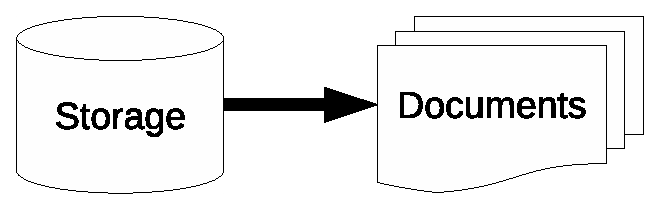
\includegraphics{Pictures/Latex_figure1.eps}
    \caption{System overview}\label{fig:figure1}
\end{figure}

All illustrations should be linked to the report via a reference in the
continuous text. Examples: ``the system is illustrated by the block schedule in
Figure~\ref{fig:figure1}'', ``According to Table x\dots'' etc. The references are
written in English beginning with a capital letter (for example ``Figure''). You
can draw your illustrations in LibreOffice Draw or any other suitable software.
LaTex will fix the numbering and you only have to do a reference to the label of
the figure.

Table 1 shows a example of a table. The table numbering behaves like the Figure
numbering. Note that the table cation is above the table. 
Table~\ref{table:methodmeasure}: Method timing measurements.

\begin{table}[ht!]
\centering
\caption{Method timing measurements.}\label{table:methodmeasure}
\begin{tabular}{c c c c}
 \midrule
  Method & Min & Max & Mean \\ [0.5ex]
 \midrule
  Method one & 10ms & 30ms & 20ms \\
 \midrule
  Method two & 20ms & 40ms & 35ms \\
 \midrule
  Method three & 50ms & 100ms & 70ms \\
 \midrule
\end{tabular}
\end{table}


\subsection{Mathematical formulas}\label{subsec:mathematicalformulas}
Mathematical formulas should be centred, or alternatively indented by
approximately a centimetre. They should be numbered, and then placed to the
right. The variable name is usually in italics. References to equations are
given with reference to the equation number, except when references are at the
start of a sentence. All variables are defined in the continuous text. See the
following examples:
The effect \(P_{i,j}\) that is transferred from base station \(i\) to the mobile
telephone \(j\) is modelled according to the following:

\begin{equation}
P_{i,j}=C \frac{P_i G_{i,j}} {d_{i,j}}
\label{eq:eq1}
\end{equation}

where is the base station broadcast effect;is the distance between the base
station and the mobile;  $\alpha$ is an exponent that is 2 in free space and
approximately 3 to 4 in a town settlement; C is a factor that depends on aerial
strengthening, channel frequency and aerial height; and is a stochastic variable
that represents the fading.

Example of reference to an equation: On the basis of Eq. (\ref{eq:eq1}) it is
realised that the received effect is proportional to the transmission effect. In
the word processing program OpenOffice, formulas can be inserted by choosing
Insert -> Object -> Formula. Formulas are numbered and referenced in the same
way as Figures and Tables using the Formula type.
